\documentclass{beamer}
\mode<presentation> {
    \usetheme{Madrid}
}
\setbeamertemplate{footline}[page number]
\usepackage{graphicx} 
\usepackage{booktabs}
\usepackage{amsmath}
\usepackage{mathtools}
\usepackage[plain]{algorithm}
\usepackage[noend]{algpseudocode}
\usepackage{multicol}

\DeclarePairedDelimiter\ceil{\lceil}{\rceil}
\DeclarePairedDelimiter\floor{\lfloor}{\rfloor}

\begin{document}
\begin{frame}
    \frametitle{Solution - A}
    \begin{figure}[h]
        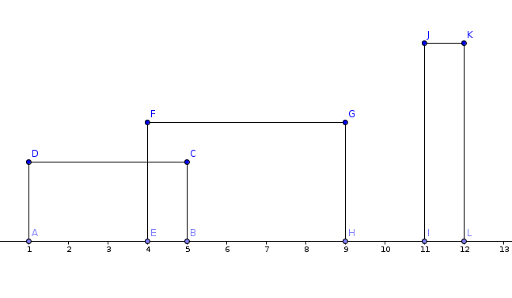
\includegraphics[scale=0.5]{sweep_line}
    \end{figure}
\end{frame}
\begin{frame}
    \frametitle{Solution - A}
\end{frame}
\begin{frame}
    \frametitle{Solution - B}
    \begin{figure}[h]
        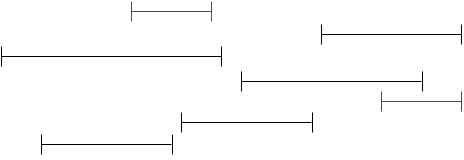
\includegraphics[scale=0.7]{interval_schedule}
    \end{figure}
\end{frame}
\begin{frame}
    \frametitle{Solution - B}
\end{frame}
\end{document} 
